\documentclass[12pt,twoside]{Z_mitthesis}

\usepackage{amsmath}
\usepackage{amssymb}
\usepackage{tikz}
\usetikzlibrary{positioning,calc,matrix}
\usepackage{makecell}
\usepackage{nicefrac}
\usepackage{datetime2}
\usepackage{sgame}
\usepackage{csquotes}
\newcommand{\tocite}{TOCITE}
\usepackage{hyperref}
\usepackage[backend=biber]{biblatex}
\usepackage{graphicx}
\usepackage{subcaption}
\usepackage{booktabs}
\graphicspath{{/Users/andreashaupt/Downloads/X_MasterThesis/tex/Figures/}}
\bibliography{/Users/andreashaupt/Documents/Writing/Bibliography/library}


\usepackage{Z_lgrind}
\usepackage{cmap}
\usepackage[T1]{fontenc}
\pagestyle{plain}
\begin{document}
\DTMnow
\title{Information Design for Platform Drivers}
\author{Andreas Haupt}
\prevdegrees{B.Sc., University of Bonn (2014) \\
M.Sc., University of Bonn (2017, 2018)\\
B.Sc., University of Frankfurt (2019)}
\department{Institute for Data, Systems, and Society}
\degree{Master of Science in Social and Engineering Systems}
\degreemonth{September}
\degreeyear{2021}
\thesisdate{August 7, 2021}
\supervisor{Jinhua Zhao}{Associate Professor}
\chairman{Fotini Christia}{Program Head, Social and Engineering Systems}
\maketitle
\cleardoublepage
\setcounter{savepage}{\thepage}
\begin{abstractpage}
With the rise of app-based matching platforms, gig workers become important suppliers of labor to transportation and food delivery. An important dimension in the management of this labor supply are pricing decisions by platforms. This thesis makes a case for the importance of another dimension of platform design for platform drivers: Demand information given to drivers. Using a large-scale survey and platform-provided data, we give evidence for the relevance of demand information for drivers' labor supply decisions. We then start our investigation into how information should be designed, and derive policy recommendations for platforms and their regulators.
\end{abstractpage}
\cleardoublepage
\section*{Acknowledgments}
I thank my family (Helga and Katrin Haupt), my roommates (Isabell, Juan-Pablo, Sophia, Salome, Bernardo) and friends and mentors (Christina, Marieke, Richard) for the emotional support I needed in this time. I thank Stephen Zoepf (Lacuna.ai, Stanford University), Ryan Green (Gridwise), Dan Calacci (MIT Human Dynamics), Xiaotong Guo (MIT Joint Transportation Lab), and Hai Wang (Singapore Management University) for helpful conversations. I thank my reader John Horton (MIT Sloan) for his open feedback. Finally, I thank my supervisor Jinhua Zhao for his visions, and for being such a kind lab leader.
\pagestyle{plain}
\tableofcontents
\newpage
\listoffigures
\newpage
\listoftables
\chapter{Introduction}\label{chap:intro}
\begin{quote}
[Gig economy,] the collection of markets that match providers to consumers on a [job] basis in support of on-demand commerce. [\dots] Prospective clients request services through an Internet-based technological platform or smartphone application that allows them to search for providers or to specify jobs. Providers (gig workers) engaged by the on-demand company provide the requested service and are compensated for the jobs. -- Congressional Information Service, \tocite
\end{quote}

See the classical \cite{Rochet2003} for competition. 

Questions of multi-homing (For Ridesharing \cite{Liu2018}, For quesitons of multi-homing \cite{Bakos2018a}, For benefits of multi-homing \cite{Belleflamme2019}, for network migration, \cite{Biglaiser2019} for platform migration, \cite{Jeitschko2014} for a model shownig captive consumers) are orthogonal to our question.

Uber highlights flexibility of drivers \cite{Uber2020}.
\section{Information Design for Platform Drivers}
This thesis studies the relevance of demand information to platform drivers and how it should be designed.

\cite{Diao2021} study the effect of ridesharing on urban mobility and find that ridesharing intensifies urban challenges. 

Preference for flexibility is documented in several studies, also empirical of nature. \cite{Angrist2017a} uses a choice experiment with virtual license plates for gig workers. Gig workers give up significant payments for working with . See also \cite{KeithChen2019}. 

By platform drivers we mean all food or grocery delivery drivers and ridesourcing drivers. While formally offering distinct services, in many urban spaces, platforms offering ridesourcing, so-called Transportation Network Companies (TNCs), also offer delivery of food or groceries. Examples of TNCs---which all offer also delivery services---are Grab and Gojek in Southeast Asian countries, Didi Yuching in China and several South American countries, as well as Uber in a large part of the world.

The Congressional Information Service's definition of gig work highlights the opportunity of search for consumers. However, it does not mention search, or any form of information acquisition by gig workers.

In most of gig work, and in particular in driving for platforms, gig workers need to make important decisions which require information or expectation on the demand for rides or deliveries: When to work, where to work, and for how long to work. Not only do these decisions have an impact on driver earning, but also on TNC operations.

Information that could affect decisions of gig workers to supply or not supply their labor often takes the form of demand information. For example, information on an area or a time period of high demand for rides can affect drivers' earnings.

This information becomes particularly crucial as platform drivers usually do not set prices for their services.


While information provision to platform driver influences decision-making of drivers, information provision becomes also important for other parts of the gig economy. For example, knowledge of demand and expectations have been demonstrated in the market for freelance software development \tocite when the market environment changed, or in investments into AirBnB housing \tocite.

This thesis focuses on the design of information to drivers. It highlights that merely considering \emph{pricing}, i.e. the setting of prices to consumers and gig workers, might be beneficially complemented by considering \emph{information provision}, both for TNC operations, a market for third-party information providers and regulation.

After positioning platform drivers in the spheres of urban transportation and the gig economy in the rest of this chapter, and reviewing important dimensions of platform design which interact with information design and information provision through third parties in \autoref{chap:literature}, we make three contributions.

The first part of our study, \autoref{chap:jakarta} investigates which other factors besides expected earnings affect driver labor supply decisions. In a large survey of platform drivers in Jakarta, Indonesia, we find significant inconsistencies with earnings maximization of drivers in terms of reported earnings, and find cultural, as well as informational aspects in drivers' labor supply decisions. We also find that drivers often do not reposition themselves, but follow the algorithm whenever possible. 

We supplement our observations on the relevance of non-pricing TNC design questions in \autoref{chap:chengdu} using earnings differences in platform-provided data. We provide an approximate value of demand knowledge using earnings differences under optimal \emph{repositioning}, i.e. movement of idle drivers to other areas in the city. We make this estimate by inferring real earnings for platform driver trips undertaken for TNC DiDi Yuching in November 2016 in Chengdu, China and comparing the earnings differences to average earnings of delivery drivers on the platform. We find that optimal repositioning, which can be seen as a very strong form of knowledge of demand, can lead to significant (at least two-fold) increase in earnings if a small group of drivers is perfectly informed about demand.

Third, we take first steps into the design of information for platform drivers in \autoref{chap:info}. In a benchmark model we formalize properties of the informational environment. We first show that never providing the same demand information to all drivers is welfare-maximizing. We show that in our model, an informational Braess' paradox arises, which is distinct from existing notions of an informational Braess' paradox.\footnote{Manxi Wu studies this in road networks; Manish Raghavan studies it for several classification technologies \tocite.} We expose that platform drivers might ignore information presented to them by the platform as a result of limited commitment of a TNC which does not allow them to credibly commit to not maximize their revenue with a choice of information. We show that third-party information aggregators can remedy this inefficiency, as can a change in the payment structure of gig drivers, and that aggregators can do so even with information provided to all subscribed drivers, as long as these are a small proportion of all drivers.

The final \autoref{chap:policy} collects policy recommendations both for TNC operators and regulators. We first show that information design is of different significance for TNC operators and regulators. While the former will need to rely on third-party aggregators to commit to disclosing information in a way that drivers will not ignore, and are in this endeavour aligned with drivers, the latter should think more carefully about equity in the proposed models: Information needs to be provided asymmetrically. While asymmetrically, it still needs to require that drivers are equally treated. We conclude with engineering challenges arising from our observations.

While we provide several facets of information design for platform drivers, we largely abstract both pricing (who pays what) and matching (which driver gets to serve which rider) decisions and competition concerns away. Real-world platforms solve joint optimization problems of pricing and information in competition with other platforms. While this means that all of our analysis needs to be seen as having a narrow view of the design possibilities of platforms, we highlight, on the contrary, that viewing platform design purely as a \emph{pricing} question might fall short of optimal mobility platform design.

Our analysis can also only be seen as mid-term, as information design to Autonomous Vehicles will depend on whether all vehicles are centrally controlled and cooperative or not. Throughout this thesis, we maintain that platform drivers are human.
\section{Background}
Platform drivers take an increasing role in urban mobility (\autoref{subsec:pdandurbanmobility}), and have special characteristics compared to other forms of gig work (\autoref{subsec:pdandgigwork}). Some of these characteristics have led to more prominent regulatory interventions into platform driving (\autoref{subsec:pdregulation}). Regulators have for the biggest part not intervened into information provision to drivers, which puts drivers into a status quo of an information environment given by their TNC apps and third parties aggregating information (\autoref{subsec:pdinfo}).
\subsection{Platform Drivers and Urban Mobility}\label{subsec:pdandurbanmobility}
As of 2021, services provided by platform drivers now make up $\nicefrac{1}{3}$ of the global taxi market \tocite. With the rise of the first transportation network companies about 15 years ago, the rapid changes leaves many of the design dimensions of this market open.

An important difference to other travel modes such as public transit is the need for dynamic rebalancing, i.e. ensuring a distribution of drivers such that in each part of the urban area expected ride demand can be met at each point in time. While dynamic rebalancing is also an important question in public transit operations, schedules can be designed with much less uncertainty.

Part of the uncertainty making dynamic rebalancing hard comes from the need to design incentives that ensure participation. Even with accurate demand models for riders, platform drivers usually have the opportunity to log off their platform or reject (some of) the rides requested by a customer. If they are not incentivized to continue working on the platform, they will not.

Incentive designs for a supply side of mobility have historically been less prominent in transportation research \tocite. This opens an opportunity for the introduction of tools used in competitive supply of labor.

\subsection{Platform Drivers as Gig Workers}\label{subsec:pdandgigwork}
Platform drivers are also gig workers \emph{qua} the definition introducing this chapter. Riders search on the platform and are matched to a driver for their ride or delivery. Nevertheless, platform drivers are extreme in some of their characteristics.

First, platform driving is, compared to other parts of the gig economy very flexible. This characteristic comes from the nature of gigs being short. Compared to other parts of the gig economy, e.g. lodging (e.g., on AirBnB, gigs usually at least one day), and services for care (e.g., care.com), technology (e.g., Andela), design (e.g., 99designs) and home services (e.g., Porch), typically require scheduling or completion within at least a day. This makes management of incentives compared to drivers


Second, the terms of the contract are fully determined by the platform. This is in contrast to other platforms such as in lodging, technology and design, where gig workers can set their own prices.

Third, reaching out to customers outside of the platform is much more challenging for platform drivers than for other gig workers. Compared to other gig work, giving a ride on the platform is short, and as both the complete contract and all payments are processed by the platform, it is hard for drivers to build gigs independently of the platform. This gives the platform additional bargaining power in negotiations with the driver.

Fourth, many of the drivers are full-time and work many hours a day. This both raises concerns over work safety, but also over wage bounds, some of which have been introduced as regulations.

\subsection{Regulation of Platform Driver Work}\label{subsec:pdregulation}
Flexibility, limitations on contracting and communication, and the ubiquity non-wage controlled, full-time work led to policy interventions regarding minimum wages and the employment status of platform drivers.

The New York City Transport and Limousine Commission introduced an earnings standard which guaranteed a \emph{proxy} minimum wage for ridesourcing drivers in New York City \cite{Parrott2018}. Drivers earn for rides an additional amount to increase the average as calibrated against historical demand data to the minimum wage level.

In 2020, California accepted via a referendum a special provision for ridesourcing drivers to be excluded from legal sufficient conditions for an employment relationship.

In contrast, the UK Supreme Court decided that ridesourcing drivers \emph{are} employees of TNCs, with labor implications for drivers, with effects for payment and insurance of dirvers.

These regulations do not include provisions on the information that drivers get from TNCs, and other actors work in this sphere.

\subsection{Platform Drivers' Payment and Information Environment}\label{subsec:pdinfo}
Most platforms drivers face an app on a smartphone, which offers them potential gigs, which they can accept or reject. At each point in time, drivers can select to log off the system, which drivers report to use strategically \tocite. In the U.S. \tocite and in our survey conducted in Jakarta (\autoref{chap:jakarta}), we find that a minority of drivers has several apps open at the same time. Hence, drivers are limited in their ability to observe demand on the other platforms.

This interacts also with payment design of platforms. Many platforms associate bonuses with the acceptance of rides, or punishments up to being blocked on the platform for not accepting ride requests. This makes being online in different platforms complicated for many drivers.

An important distinction will be three time periods, which we call, in accordance with nomenclature introduced by Uber \tocite \emph{phases 1, 2, and 3}.

Phase 1 corresponds to times where the driver is online but idle. In these times, the driver is not sent ride requests and does (except for bonus payments for repositioning) not earn money.

Phases 2 and 3 refer to the time between the acceptance of a ride request and the pickup of the passenger, and the ride, respectively. In these phases, riders are paid.

The goal of this thesis is to establish the relevance of providing drivers with demand information, and will only significantly affect driver behavior in phase 1. Drivers that are picking up or driving a rider have a clear task, and even a contract for their work. The main question we ask in our theoretical section will be when the platform can transmit any information that will not be ignored.

\chapter{Related Work}\label{chap:literature}
Our work at the intersection of the Labor Economics in the Gig Economy, Supply Management in Transportation, Information Design, and information gathering from platforms contributes to several literatures.
\section{Estimating Labour Supply Through Surveys}
Our contribution first contribution, a survey to platform drivers in Jakarta, Indonesia, uses a survey to study the labor supply decisions of drivers, and does so using a survey.
\subsection{Models of Platform Driver Labour Supply}
Labor supply choices of drivers, or more generally participation decisions in two-sided platforms, is assumed as exogenous, or rational expectations of drivers is assumed.

Papers showing the impact of multi-homing use either stylized models such as those inspired by Hotelling lines \cite{bryan2019theory,bakos2020platform}, assume exogenous models of \cite{castillo2017surge} or do not model multi-homing decisions \cite{liu2017impact}.

Other papers assume that in moments where agents join a platform, they have exact knowledge of the surplus that is gained and the prices that both sides receive \cite{liu2019multihoming}.

\cite{Wang_Yang_2019} offers a comprehensive review on the ride-hailing system including demand, supply and platform perspectives. 
Driver behavior is modeled differently in the ride-hailing literature.   
Regarding operations and optimizations for ride-hailing platforms, e.g., driver-customer matching, idle vehicle rebalancing and vehicle routing, drivers are assumed to follow the instructions of platforms~(\cite{Bertsimas_Jaillet_Martin_2019, Alonso-Mora_2017, Braverman_Dai_Liu_Ying_2019, Wen_Zhao_Jaillet_2017}).

Simple driver behavior models are proposed in the pricing literature of the ride-hailing system. 
\cite{Bai_So_Tang_Chen_Wang_2019} propose a queuing model to optimize platforms' profit while considering price-sensitive customers and earning-sensitive drivers. Each driver has a reservation earning rate based on his outside option and the driver will provide services only if earning rate exceeds the reserved value.
\cite{Taylor_2018} evaluate the impact of uncertainty in passenger delay sensitivity and driver independence on platforms' optimal per-service price and wage. Each driver has an opportunity cost and the driver will participate in the platform when having non-negative expected utility. 

To better understand driver behavior, several studies discuss the general reasons why drivers work in the ride-hailing system.
An econometric framework with closed-form measures is proposed by \cite{Sun_Wang_Wan_2019} to estimate both the participation elasticity and working-hour elasticity for drivers. In particular, this article assumes that there 
\cite{Chaudhari_Byers_Terzi_2018} design an earnings-maximization strategy for drivers and show that strategic behavior about when and where to drive have significant impact on drivers' earnings.
\cite{Jiang_Kong_Zhang_2021} show that regret aversion and ignorance of suggestion are the two major behavioral factors which influence drivers' re-positioning decisions.
\subsection{Labour Economics and Industrial Economics}
Our analysis in \autoref{chap:jakarta} pertains to 

\section{Investigations into Platform Pricing}
To understand platform pricing, many platforms 
\subsection{Scraping-Based Studies}
Some platforms scrape data from platforms, such as studies on platform competition in New York \tocite (rosaia) and a consumer surplus comparison of taxi and ridesourcing \tocite (shapiro). Similarly, \tocite (peaking under the hood) uses large-scale simulation of apps.
\subsection{Information from Platforms}
\subsection{Gathering Driver Data}
\section{Driver Repositioning}
The repositioning of drivers, also known as Dynamic Rebalancing in the literature on platform design. 
\section{Cheap Talk and Information Design}
Our third contribution contributes to a line of work on cheap talk and information design. 
\subsection{Cheap Talk}
The standard model of Crawford-Sobel \tocite, in which one agent, which has a piece of information, communicates with another agent, who can take an action affecting both agents' utility, too strong mismatch of incentives leads to no communication. A classical model of cheap talk, communication is costless, and does neither binds sender nor receiver to take a particular action in the future \tocite (Farrell). In our first model of information provision, we model the strategic interaction between the platform and drivers as a cheap talk game, and show that if the incentives of the platform and drivers diverge sufficiently, that, in equilibrium, no information is transmitted, in terms of the cheap talk literature, the platform \emph{babbles}.
\subsection{Bayesian Persuasion and Information Design}
In contrast to cheap talk, Information Design models allow the sender to commit to rules for which information they reveal \tocite (kamenica gentzkow, also annual reviews). This can have profound implications for the outcome compared to Cheap Talk. This will also be a feature in our model in \autoref{chap:infodesign}. 

\subsection{Information and Mechanism Co-Design}
While we consider a pure mechanism design problem, work on the co-design of mechanisms and information, such as \tocite(mechanism design with aftermarkets). This paper considers the informational effect of allocations. In our platform driver setting this would model the informational effect of surge prices for rational drivers.
\chapter{Platform Driver Labor Supply Beyond Earnings Maximization}\label{chap:jakarta}
\begin{quote}
Since Uber’s introduction in 2009, ridesharing platforms like Uber, Didi, Grab, and Lyft have radically transformed the taxi and limo industry. These services, which allow consumers to order a car to their location via a smartphone application, now control roughly 1/3 of the international taxi market. In other words, a ridesharing firm acts as a platform matching drivers to riders and setting the pricing terms between them. ---\cite{Bryan2019a}
\end{quote}
 This chapter analyzes data from a survey in Jakarta and shows that drivers do not purely maximize their earnings in their labor supply choices. In an analysis of free-text answers, we highlight understanding of the app and information as important determinants of driver behavior.
\section{Survey}
Our data comes from a survey conducted in spring 2021 in Jakarta, Indonesia.
\subsection{Sample}
Participants were asked to complete an online survey hosted on Qualtrics. 846 complete survey responses were submitted. We excluded from the analysis drivers that stated more than 16 hours of work per day and stated earnings smaller than 10,000 IRB or larger than 2,000,000 IRB. The survey participants were recruited through social media (platform driver WhatsApp groups).

Figure \ref{fig:age} shows the age distribution of participants, where around 50\% of drivers are within the age group of 30 to 39. Figure \ref{fig:gender_mode_driver} reveals that over 97\% of drivers who participated in the survey are male and around 97\% are motorbike (delivery) drivers. 

Three major ride-hailing companies operate in Jakarta: Grab, GoJek and Shopee. While Grab and GoJek are incumbents in this market, Shoppee entered the market only in 2021. Figure \ref{fig:platform} shows the percentage of drivers working for each of the platforms, double-counting multi-homers. Around 94\% of drivers work for the incumbents Grab or GoJek. In our sample of drivers, only 12\% of drivers questioned in the survey are multi-homers.
\begin{figure}[!ht]
    \centering
    \includegraphics[width=10cm]{platform.png}
    \caption{Platform distribution of drivers. (GoJek: 60\%, Grab: 34\%, Shopee: 6\%)}
    \label{fig:platform}
\end{figure}  
 \begin{figure}[!ht]
      \centering
      \begin{subfigure}[b]{0.49\textwidth}
          \centering
          \includegraphics[width=\textwidth]{age.png}
          \caption{Age distribution of drivers. (Below 20: 2\%, 20 to 29: 27\%, 30 to 39: 49\%, 40 to 49: 20\%, above 50: 3\%)}
          \label{fig:age}
      \end{subfigure}
      \hfill
      \begin{subfigure}[b]{0.49\textwidth}
          \centering
          \includegraphics[width=\textwidth]{gmd.png}
          \caption{Gender, mode and driver type distributions of drivers. (Male: 97\%, female: 3\%; motorbike: 97\%, car: 3\%; single-homer: 88\%, multi-homer: 12\%) }
          \label{fig:gender_mode_driver}
      \end{subfigure}
         \caption{Sociodemographic information and driving behaviors of survey participants.}
         \label{fig:survey_stats}
 \end{figure}
\subsection{Questions}
 The survey consists of multiple questions blocks and is reproduced in its entirety in Appendix~\ref{appendix:survey}. 

In a first block, participants were asked to check all TNCs they have worked for in the past 30 days. A survey respondent is defined as a \emph{multi-homer} if they have been working for at least two platforms in the past 30 days. In this first block, basic information and driving behavior are asked as well, e.g., vehicle type used, previous occupation, behaviors while waiting for the next order.

The second block's questions differ for multi-homers and non-multi-homers. Multi-homers are asked how they switch between different platforms, allocations of their working hours and reasons for multi-homing. For non-multi-homers, reasons for non-multi-homing and factors that would make them multi-home are elicited.

In a third block, for each ride-hailing platform survey participants have worked for in the last 30 days, respondents are asked questions about their labor supply choices. Type of work (delivery, ridesourcing), part of the city of highest activity, and daily working hours, distance, and earnings.

A final block elicited socio-demographic information, including age, gender, educational status, income level, living areas, and weekly expenses. 
\section{Descriptive Evidence}
A first observation we make is that there is significant correlation between experience working as a taxi driver before and multi-homing behaviors. The OLS regression model shown in Table \ref{tab:opang} suggests that drivers who has been motorcycle taxi drivers before are less likely to multi-home in Jakarta market.
 \begin{table}
 \centering
     \caption{Results of regression models predicting multi-homing behaviors of ride-hailing drivers in Jakarta based on previous occupation}
         \begin{tabular}{lcccccc}
         \toprule
         \textbf{Variable} & \textbf{coef} & \textbf{std err} & \textbf{t} & \textbf{P$> |$t$|$} & \textbf{[0.025} & \textbf{0.975]}  \\
         \midrule
         \textbf{Intercept} &       0.1276***  &        0.012     &    10.735  &         0.000        &        0.104    &        0.151     \\
         \textbf{Former taxi driver}     &      -0.0796**  &        0.031     &    -2.574  &         0.010        &       -0.140    &       -0.019     \\
         \midrule
         \multicolumn{1}{r}{\textbf{R-squared: }}   & 0.008 & \multicolumn{3}{c}{\textbf{Adjusted R-squared: }}  & 0.007 & \\
         \bottomrule 
         \end{tabular}
     \label{tab:opang}
 \end{table}

 Finally, we turn our attention to the results of our regression models exploring the impact of being a part-time ride-hailing driver on drivers' multihoming behaviors.
 
 From the model results shown in Table \ref{tab:part-timer}, we find that part-time ride-hailing drivers are more likely to multi-home in our sample. However, it is a less significant predictor of multihoming behaviors compared to other variables above.

 \begin{table}
 \centering
     \caption{Results of regression models predicting multi-homing behaviors of ride-hailing drivers in Jakarta based on whether being part-time ride-hailing drivers}
         \begin{tabular}{lcccccc}
         \toprule
         \textbf{Variable} & \textbf{coef} & \textbf{std err} & \textbf{t} & \textbf{P$> |$t$|$} & \textbf{[0.025} & \textbf{0.975]}  \\
         \midrule
         \textbf{Intercept}                           &       0.1097***  &        0.012     &     9.258  &         0.000        &        0.086    &        0.133     \\
         \textbf{Part-Time} &       0.0441  &        0.032     &     1.384  &         0.167        &       -0.018    &        0.107     \\
         \midrule
         \multicolumn{1}{r}{\textbf{R-squared: }}   & 0.002 & \multicolumn{3}{c}{\textbf{Adjusted R-squared: }}  & 0.001 & \\
         \bottomrule 
         \end{tabular}
     \label{tab:part-timer}
 \end{table}
 \subsection{Earnings for Different Platforms}
Our main finding concerns the earnings for different platforms. Figure \ref{fig:hourly_salary} displays the hourly salary distribution of all survey respondents in Jakarta. The median respondent makes less than 20,000 IRB (approximately 1.4 USD) per hour, which is significantly less than the average hourly salary 120,175 IRB (approximately 8.4 USD) in Jakarta~\cite{Jakarta_hourly_salary}. This stands even when controlling for sociodemographics.

 \begin{figure}
     \centering
     \includegraphics[width=0.6\textwidth]{hourlysalary.png}
     \caption{Hourly salary distribution of survey respondents (ride-hailing drivers in Jakarta)}
     \label{fig:hourly_salary}
 \end{figure}

We estimate, among all single-homers, the correlation between working for GoJek and hourly salary in Table \ref{tab:hourly_salary}. We exclude the 3\% of non-motorcycle drivers due to their significantly different earnings. The model results suggest that GoJek drivers earn significantly less than drivers from other platforms, 11,000 IRB (approximately 0.77 USD) less per hour. While a weak effect ($R^2 = 0.002$), it is significant.

\begin{table}[!htbp] \centering
\begin{tabular}{@{\extracolsep{5pt}}lcc}
\\[-1.8ex]\hline
\hline \\[-1.8ex]
& \multicolumn{2}{c}{\textit{Dependent variable:}} \
\cr \cline{2-3}
\\[-1.8ex] & (1) & (2) \\
\hline \\[-1.8ex]
 Intercept & 30713.817$^{***}$ & 32141.158$^{***}$ \\
  & (1927.295) & (10919.276) \\
 Q54[T.30 - 39] & & 599.344$^{}$ \\
  & & (9829.024) \\
 Q54[T.30 - 39]:Q58[T.Yes] & & -1459.150$^{}$ \\
  & & (10215.505) \\
 Q54[T.40 - 49] & & -5300.705$^{}$ \\
  & & (13705.572) \\
 Q54[T.40 - 49]:Q58[T.Yes] & & 2649.267$^{}$ \\
  & & (14135.068) \\
 Q54[T.Above 50] & & -655.081$^{}$ \\
  & & (17545.153) \\
 Q54[T.Above 50]:Q58[T.Yes] & & 3628.347$^{}$ \\
  & & (19003.614) \\
 Q54[T.Under 20] & & -689.077$^{}$ \\
  & & (4819.356) \\
 Q54[T.Under 20]:Q58[T.Yes] & & -689.077$^{}$ \\
  & & (4819.356) \\
 Q55[T.Male] & & -5813.134$^{}$ \\
  & & (4617.561) \\
 Q55[T.Prefer not to answer] & & -17966.204$^{}$ \\
  & & (19349.857) \\
 Q57[T.None of the above] & & -0.000$^{}$ \\
  & & (0.000) \\
 Q57[T.S1 or higher] & & -5956.143$^{}$ \\
  & & (7460.034) \\
 Q57[T.SD] & & 6745.220$^{}$ \\
  & & (8008.309) \\
 Q57[T.SMA] & & -338.772$^{}$ \\
  & & (5669.506) \\
 Q57[T.SMP] & & 1058.908$^{}$ \\
  & & (6598.707) \\
 Q58[T.Yes] & & 5170.436$^{}$ \\
  & & (8691.783) \\
 gojek[T.True] & -11001.520$^{***}$ & -10506.619$^{***}$ \\
  & (2366.886) & (2426.682) \\
\hline \\[-1.8ex]
 Observations & 552 & 552 \\
 $R^2$ & 0.038 & 0.052 \\
 Adjusted $R^2$ & 0.036 & 0.025 \\
 Residual Std. Error & 26284.803(df = 550) & 26435.066(df = 536)  \\
 F Statistic & 21.605$^{***}$ (df = 1.0; 550.0) & 1.942$^{**}$ (df = 15.0; 536.0) \\
\hline
\hline \\[-1.8ex]
\textit{Note:} & \multicolumn{2}{r}{$^{*}$p$<$0.1; $^{**}$p$<$0.05; $^{***}$p$<$0.01} \\
\end{tabular}
\caption{Results of regression models predicting hourly earnings of platform drivers drivers in Jakarta based on whether working for GoJek}\label{tab:working_hours}
\end{table}


For the same group of drivers, we consider the difference of total working hours between ride-hailing platforms.
 The model results in Table \ref{tab:working_hours} show that GoJek drivers work significantly longer than drivers from other platforms, 1.0335 hours more per day.
 Both regression results imply that there existing a large switching cost between GoJek and other platforms (Grab and Shopee) in Jakarta ride-hailing market. 
 
 GoJek motorcycle drivers work longer hours but earn less compared to other drivers. We use Natural Language Processing tools to gain additional insights on what, besides earnings maximization, might drive the choices to work for Grab as compared to GoJek.

 
 
 \begin{table}[!htbp] \centering
\begin{tabular}{@{\extracolsep{5pt}}lcc}
\\[-1.8ex]\hline
\hline \\[-1.8ex]
& \multicolumn{2}{c}{\textit{Dependent variable:}} \
\cr \cline{2-3}
\\[-1.8ex] & (1) & (2) \\
\hline \\[-1.8ex]
 Intercept & 10.664$^{***}$ & 8.328$^{***}$ \\
  & (0.162) & (0.874) \\
 Q54[T.30 - 39] & & -0.761$^{}$ \\
  & & (0.791) \\
 Q54[T.30 - 39]:Q58[T.Yes] & & 0.970$^{}$ \\
  & & (0.829) \\
 Q54[T.40 - 49] & & -1.880$^{*}$ \\
  & & (1.072) \\
 Q54[T.40 - 49]:Q58[T.Yes] & & 1.916$^{*}$ \\
  & & (1.116) \\
 Q54[T.Above 50] & & -1.056$^{}$ \\
  & & (1.440) \\
 Q54[T.Above 50]:Q58[T.Yes] & & 1.595$^{}$ \\
  & & (1.572) \\
 Q54[T.Under 20] & & 1.204$^{}$ \\
  & & (2.642) \\
 Q54[T.Under 20]:Q58[T.Yes] & & -2.903$^{}$ \\
  & & (2.785) \\
 Q55[T.Male] & & 0.928$^{**}$ \\
  & & (0.395) \\
 Q55[T.Prefer not to answer] & & 1.378$^{}$ \\
  & & (1.523) \\
 Q57[T.None of the above] & & -0.000$^{}$ \\
  & & (0.000) \\
 Q57[T.S1 or higher] & & -0.198$^{}$ \\
  & & (0.603) \\
 Q57[T.SD] & & 0.073$^{}$ \\
  & & (0.698) \\
 Q57[T.SMA] & & -0.032$^{}$ \\
  & & (0.480) \\
 Q57[T.SMP] & & 0.063$^{}$ \\
  & & (0.568) \\
 Q58[T.Yes] & & 1.749$^{**}$ \\
  & & (0.689) \\
 gojek[T.True] & 1.033$^{***}$ & 0.866$^{***}$ \\
  & (0.210) & (0.206) \\
\hline \\[-1.8ex]
 Observations & 655 & 655 \\
 $R^2$ & 0.036 & 0.136 \\
 Adjusted $R^2$ & 0.034 & 0.114 \\
 Residual Std. Error & 2.648(df = 653) & 2.536(df = 638)  \\
 F Statistic & 24.120$^{***}$ (df = 1.0; 653.0) & 6.273$^{***}$ (df = 16.0; 638.0) \\
\hline
\hline \\[-1.8ex]
\textit{Note:} & \multicolumn{2}{r}{$^{*}$p$<$0.1; $^{**}$p$<$0.05; $^{***}$p$<$0.01} \\
\end{tabular}
\caption{Results of regression models predicting daily working hours of ride-hailing drivers in Jakarta based on whether working for GoJek}\label{tab:hourly_salary}
\end{table}

\section{Free-Text}
 In this section, we use a topic model (Latent Dirichlet Analysis) to discover potential non-monetary reasons for the choice of TNC that drivers work for. All of the analysis is use answers to question 16 (compare Appendix~\ref{appendix:survey}) \enquote{Anything else we should know about why you decided not to use multiple platforms?}.

We fine-tuned a natural language model BERT \cite{Devlin2019} trained on the Indonesian Wikipedia to predict the choice of platform worked for based on the answer to question 16. We list global feature importance in our training data set for the prediction of the platform in \autoref{tab:free-text}.

The words most indicative of working for GoJek, the platform with lower reported earnigns, are

\begin{table}
\begin{tabular}{ccc}
\toprule
&&\\
\midrule
&&\\
\bottomrule	
\end{tabular}
\caption{Sum of Feature Importance in SHAP scores}	
\end{table}


%TODO: FInish analysis.
%Potential things to see:
%gridwise: Using across platforms
%vehicle requirements
%bounced out
%focus/confusion
%indonesian incumbent
\section{Discussion}
We find significant earnings and working hours differences between single-homing drivers. The majority of respondents works for a platform where they report longer working hours and less hourly wages.

In our analysis of free-text answers, we find that drivers working for a lower-paying platform cite more frequently reasons for %TODO: Finish this.

This gives introductory evidence for features beyond matching and pricing, relating to the informational environment of drivers. The value of demand information, whose design we are going to study in \autoref{chap:infodesign} is part of our analysis the next chapter.
 \section{Conclusion}

\chapter{The Value of Information}\label{chap:chengdu}
While the last chapter investigated stated aspects of relevance for labor supply, this section shows the \emph{potential} effects of platform design beyond matching and pricing.

In this chapter, we give evidence that demand information can significantly increase earnings for platform drivers. The earnings gains are aligned with claims by companies that offer information services to drivers such as Gridwise or the Mileage tracker that additional information can increase earnings. We first describe data that we use in \autoref{sec:chengdudata}, we then estimate driver earnings in optimized repositioning in \autoref{sec:chengduestimation} and close with comparing this with driver income under non-optimized behavior and discuss our results in \autoref{sec:chengdudiscussion}.
\section{Description of Data}\label{sec:chengdudata}
The DiDi KDD Challenge 2020, sponsored by DiDi Yuching, consisted of two challenge. An order dispatch challenge, and a driver repositioning challenge. We will work with data and submissions of the latter.

\subsection{Annotated Order Data}
We use a dataset of 14,131,874 orders dispatched in Chengdu, China, in November 2016. An order consists of an origin-destination pair, a timestamp for beginning and end, an identifier for the driver that took the order, and a number of \emph{reward units}. As the data is not publicly available anymore, we are unable to provide replication data for the following analysis.

A main challenge in our analysis is to recover the number of reward units corresponding to a RMB. Given our estimation below, we can transfer repositioning scores to monetary values, which gives us an estimate of 

\subsection{Evaluation in Paper}
The KDD 2020 reinforcement learning challenge solves an optimal repositioning problem together with an optimal order dispatch problem. The problem is a partial observed semi-Markov Decision Process. In Reinforcement Learning language, which we review in \autoref{app:math}.

The system's observable state for the order dispatch algorithm consists of a list of orders to be dispatched at each point in time. This means a list of origin-destination pairs for orders, and for each driver timestamps of \emph{estimated} order pickup and arrival times, as well as the distance for the driver. The reinforcement learning algorithm's actions are matchings of drivers to orders, the challenge does not consider carpooling. Orders need to be dispatched within two seconds, otherwise they are lost. (We specify the complete environment in \autoref{app:kdd}. As part of the state transitions, there is estimated data for cancellation probabilities when sending a driver to pick up orders from different locations.

The objective in the order dipatch algorithm is to maximize average driver income, which, as the system does not model drivers logging off strategically, is proportional to the total driver revenue in terms of orders completed.

The system's observable state for the driver repositioning challenge, which we are most interested in, consists of a set of drivers to be repositioned. There is a targeted group of drivers, which, after their first five minutes of being idle move according to historical transition probabilities between regions, can be repositioned. In addition to a timestamp, the only information given on drivers is a coarse position on a hexagonal grid of the urban area of Chengdu. The actions are, for each driver to be repositioned, a destination location. Agents are then repositioned at 3m/s in the spherical/great arc distance.

The objective in the driver repositioning problem is to maximize mean driver income rate for drivers. Denote $J_k^n (\pi)$ the online time for driver $k$ at day $n$ in hours.\footnote{While the existing documentation do not specify the unit of this measure, our calculations below show that assuming online time is measured in hours leads to correct results.} Denote driver $k$'d income on day $n$ under policy $\pi$. For the set of all targeted drivers $K$ and days $N$, the goal of the challenge was to maximize
\[
	\frac{1}{\lvert K\rvert} \sum_{k \in K} \frac{\sum_{n \in N} J_k^n (\pi)}{\sum_{n \in N} L_k^n (\pi)}.
\]

We claim that the optimal repositioning score for drivers can give insight into the value of information for these drivers, as long as there are not too many of them.

If drivers have sufficient information about the demand throughout the city, they can reposition themselves to another location in expectation of getting higher earnings. As the maximization takes into account all online time, in particular the time moving to another area of the city, the earnings increase from a performant repositioning algorithm in this challenge can also be seen as a proxy for earnings of informed drivers.

In this argument, the small number of repositioned drivers is important. A challenge for drivers, but not for the platform, is that a knowledge on high demand in some area might lead to congestive effects---too many drivers enter high-demand areas.

But even with more drivers, private messages, which we discuss in \autoref{chap:infodesign} help. Private messages is demand information (or, as we show, equivalently recommendations of to which area to move) only given to particular drivers, solving their 

\subsection{Earnings Table}
We are using a publicly available table for earnings from 2021. In 2017, DiDi introduced two tiers of service for their drivers, Express and Premium. After personal conversations with experts, we use the table for express, reproduced in \autoref{tab:earnings}. 

The earnings table contains, dependent of the time of the day, a base price $b_t$, earnings per kilometer $l_t$ and minute driven $d_t$. At the time of the data, November 2016, additionally, a surge multiplier $s_t$. The total earnings $e_t$ for a ride of $L$ kilometers and duration $D$ are given by 
\begin{equation}
	e_t = s_t(b_t + l_t L + d_t D).\label{eq:earnings}
\end{equation}
\begin{table}[]
\centering
\begin{tabular}{lllll}
\toprule
 & Base Price & Price/km & Price/min &  \\
\midrule
$22:00-07:00$  & 12.40      & 2.70     & 0.48      &  \\
$07:00-10:00$  & 12.40      & 2.55     & 0.48      &  \\
$10:00-16:00$ & 11.40      & 1.95     & 0.42      &  \\
$16:00-19:00$ & 12.40      & 2.33     & 0.48      &  \\
$19:00-22:00$ & 11.40      & 1.95     & 0.42      & \\
\bottomrule
\end{tabular}
\caption{Earnings for express drivers}
\end{table}
\section{Estimation}\label{sec:chengduestimation}
We assume in the following that reward units are a constant multiple of RMB. The underlying assumption is the following proposition.

\begin{prop}
	Assume that reward units $r$ are a function $f$ of the earnings from an order in RMB. Assume that any policy generated for reward units is also optimal for policies in RMB. Then, the function $f$ is a constant multiplication, $f(x) = cx$ for some $c > 0$.
\end{prop}

\subsection{Regression}\label{subsec:chengduregress}
We assume that a negligible fraction of rides uses a surge price and therefore estimate an equation simplifying \eqref{eq:earnings},
\[
	e_t = b_t + l_t L + d_t D.
\]
Our estimate of time is the times given in the order data. We use the Google Maps API to estimate distance in driving. The estimation results are presented in \autoref{tab:rewardunits}. We find highly significant and consistent estimates on the coefficients for distance and duration.

\begin{table}[!htbp] \centering
\begin{tabular}{@{\extracolsep{5pt}}lcc}
\\[-1.8ex]\hline
\hline \\[-1.8ex]
& \multicolumn{2}{c}{Dependent variable: Reward Units} \
\cr \cline{2-3}
\\[-1.8ex] & (1) & (2) \\
\hline \\[-1.8ex]
 Intercept & 0.751$^{***}$ & 0.703$^{***}$ \\
  & (0.042) & (0.041) \\
 distance & 0.290$^{***}$ & 0.317$^{***}$ \\
  & (0.014) & (0.076) \\
 duration & 0.065$^{***}$ & 0.116$^{***}$ \\
  & (0.005) & (0.041) \\
 hour[T.22-7]:distance & & -0.043$^{}$ \\
  & & (0.077) \\
 hour[T.22-7]:duration & & -0.050$^{}$ \\
  & & (0.041) \\
 hour[T.7-10]:distance & & -0.067$^{}$ \\
  & & (0.089) \\
 hour[T.7-10]:duration & & -0.037$^{}$ \\
  & & (0.043) \\
 hour[T.offhour]:distance & & 0.003$^{}$ \\
  & & (0.078) \\
 hour[T.offhour]:duration & & -0.057$^{}$ \\
  & & (0.041) \\
\hline \\[-1.8ex]
 Observations & 3,997 & 3,997 \\
 $R^2$ & 0.883 & 0.894 \\
 Adjusted $R^2$ & 0.883 & 0.894 \\
\hline
\hline \\[-1.8ex]
\textit{Note:} & \multicolumn{2}{r}{$^{*}$p$<$0.1; $^{**}$p$<$0.05; $^{***}$p$<$0.01} \\
\end{tabular}
\end{table}
We observe that much of the variance can be explained by our model ($R^2 = 0.887$). As another sanity check, we infer the distribution of surge prices throughout the day. 
\section{Discussion}\label{sec:chengdudiscussion}
We see that optimal driver repositioning has a significant effect on driver earnings if only a few drivers are treated to this additional information. 

In a model with more drivers being treated, informed drivers might \emph{crowd out} each other, and earnings differential might be smaller.

This does not mean that information design is not possible to improve platforms, but that, for each trip, only a subset of drivers may be informed of it. This robust property is one of our findings in the next chapter.
\chapter{Information Design}\label{chap:infodesign}
\begin{quote}
	The information design problem has
a literal interpretation: there
really is an information designer (or mediator, or sender) who can commit to provide extra information to players to serve her own
interests. While the commitment assumption may be problematic in many settings, it provides a useful benchmark.--\tocite
\end{quote}
In this section, we study pure information design for platform drivers. We refer to it as \emph{pure} as we study information provision while keeping the pay to drivers fixed. Part of our conclusions in this section are that for sufficiently high non-internalized costs from the platform, pure information design will lead to no information transmission to drivers in equilibrium.
\section{Model}
In our stylized model, two agents simultaneously decide to drive to a part of a city or to do something else. The platform observes, or has a better estimate on the demand state $\theta \in \{0,1\}$. Before each of the drivers makes her decision on whether to drive, the system can send a message $m_1$ to driver $1$ and $m_2$ to driver $2$ on whether there is demand on the platform. Drivers get utility $1$ if they get an order, and incur a cost of driving to the location of $\varepsilon$. This gives a game table in \autoref{fig:twodrivers}. 

The platform gets utility of $1$ if at least one of the drivers gets to the desired location, and $0$ utility otherwise. The divergence of platform and driver utility stems from the payment structure for drivers, as we described in the introduction: Drivers only get paid for phase 2, when they are matched to a ride.

The platform can send messages to drivers. The platform can either send a message to drivers without committing to any particular form of information revelation (\autoref{subsec:infodesign}) such as \enquote{I recommend you to go to this place, and I will not recommend this to others}, or does not have the power to credibly commit to this (\autoref{subsec:cheaptalk}). 

\begin{figure}
\centering
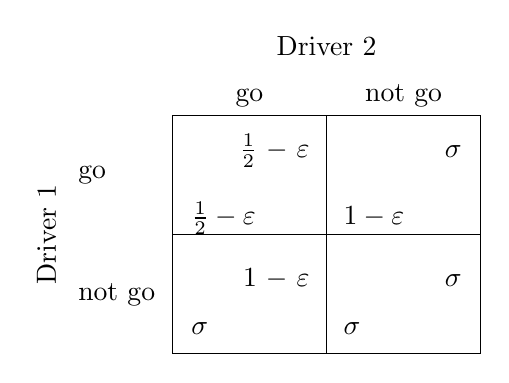
\begin{tikzpicture}
\matrix[matrix of math nodes,every odd row/.style={align=right},every even row/.style={align=left},every node/.style={text width=1.5cm},row sep=0.2cm,column sep=0.2cm] (m) {
$\frac12-\varepsilon$&$\sigma$\\
$\frac12-\varepsilon$&$1-\varepsilon$\\
$1-\varepsilon$&$\sigma$\\
$\sigma$&$\sigma$\\
};
\draw (m.north east) rectangle (m.south west);
\draw (m.north) -- (m.south);
\draw (m.east) -- (m.west);
\coordinate (a) at ($(m.north west)!0.25!(m.north east)$);
\coordinate (b) at ($(m.north west)!0.75!(m.north east)$);
\node[above=5pt of a,anchor=base] {go};
\node[above=5pt of b,anchor=base] {not go};

\coordinate (c) at ($(m.north west)!0.25!(m.south west)$);
\coordinate (d) at ($(m.north west)!0.75!(m.south west)$);
\node[left=2pt of c,text width=1cm]  {go};
\node[left=2pt of d,text width=1cm]  {not go};

\node[above=18pt of m.north] (firm b) {Driver 2};
\node[left=1.6cm of m.west,rotate=90,align=center,anchor=center] {Driver 1};
\end{tikzpicture}
\caption{Payoff Matrix for the two-driver game.}\label{fig:twodrivers}
\end{figure}
\subsection{Cheap Talk}\label{subsec:cheaptalk}
In cheap talk, the platform discloses some information to a driver, which, given the update, updates their behavior. More concretely, there is an abstract set of \emph{messages} $m \in \mathcal M$ that the platform can send. The players receive the message and play optimally. In particular, the timeline of the game is:
\begin{enumerate}
	\item The demand $\theta$ at the area is realized.
	\item The platform decides to send messages $(m_1, m_2)$ to the drivers.
	\item The drivers decide to drive or not drive to the area.
	\end{enumerate}
We solve for perfect Bayesian (signalling) equilibria of this game.
\begin{theorem}
	In the cheap talk model, Perfect Bayesian equilibria have the following form:
	\begin{enumerate}
		\item If $\sigma < \frac12 - \varepsilon$ or $\sigma > 1-\varepsilon$, then the platform is indifferent between any message, the drivers will go to the area or not go to it.
		\item If $\sigma $
	\end{enumerate}
\end{theorem}
If the general outside option is very low ($\sigma < \frac12 - \varepsilon$) or very high ($\sigma > 1 - \varepsilon$), drivers go to the area in hope to get a ride or stay away from it, respectively, even without demand information. The platform is indifferent between any demand information given that it won't influence the driver's decisions.

For an intermediate outside option ($\frac12 - \varepsilon < \sigma < 1 - \varepsilon$), the 




In this environment, hence, if the not internalized cost from 



\subsection{Information Design}\label{subsec:infodesign}
In information design, the drivers can commit to a driver 
\subsection{Public and Private Messages}
\section{Inefficiencies}
In this environment, two sources of in
\subsection{Inefficiencies through lack of commitment}
\subsection{Inefficiencies through public information}

\section{Remedies}
Given the inefficiencies observed in the last section, some remedies for the market should be considered. We propose that 
\subsection{Commitment via third parties}
\subsection{Commitment via reputation}
\subsection{Approximate Efficiency of Public Information to Few Drivers}
\chapter{Conclusion and Policy Implications}\label{chap:policy}
This thesis studied the relevance and optimal design of information provided to ridesourcing drivers. \autoref{chap:jakarta} showed that besides earnings maximization, drivers also take into account cultural and infromational considerations in their labor supply decisions. \autoref{chap:chengdu} showed that there are high potential earnings gains from additional information. We then went on to study commitment and privacy of messages as two challenges. In this last chapter, we consider three stakeholder groups, platforms, regulators and transportation engineers with policy recommendations and additional complications arising out of this work. 
\section{The Commitment Challenge for Platforms}
We observed in \autoref{chap:infodesign} that the limited commitment of the platform to providing different platform can lead to not information being transmitted and we proposed reputation 
\section{The Fairness Challenge for Transportation Regulators}
\section{Challenges for Transportation Engineers}
The above two challenges give interesting challenges for transportation engineers.
\subsection{Allowing for Commitment without Harming Businesses}

\subsection{Managing Fairness in Information Provision}
\appendix
\input{X1_survey}
\chapter{Complete Earnings Information for DiDi Platform Drivers}
In this brief appendix, we reproduce payment information for platform drivers.
\chapter{Omitted Proofs}\label{app:omitted}
\chapter{Mathematical Background}

\section{On Markov Decision Processes}
Here we introduce a notation on Markov Decision Processes
\section{On Statistical Experiments and Bayes-Correlated Equilibria}
\input{X_tables}
\input{X_figures}
\begin{singlespace}
\printbibliography
\end{singlespace}
\end{document}